\section{Numerical results}

\subsection{Gaussian potential}

To validate our implementation, we will calculate total energy of a system with
attractive "ionic" potential which has the following general form:
\begin{equation}
V_{\mathrm{ion}}(r) = -A\exp(-\alpha r^2)
\end{equation}
where $A$ and $\alpha$ are positive constants.
We compare the obtained electronic total energy using the one obtained by
\textsc{Octopus} program \cite{Marques2003,Castro2006,Xavier2015}
which implements finite difference approaches to solve Kohn-Sham equations.
 
The calculations are done using $16 \times 16 \times 16$ bohr periodic unit cell
and the center of the potential is set to be the center of the cell, i.e.
at coordinate $(8,8,8)$ bohr. The value of $A$ is set to 10 and we use 4 different
values of $\alpha$, i.e. 0.5, 1.0, 2.0, and 3.0. The visualization of the potential
is shown in Figure \ref{fig:gauss_pot}. Notice that the potential becomes sharper
as value of $\alpha$ becomes larger.
\begin{figure}
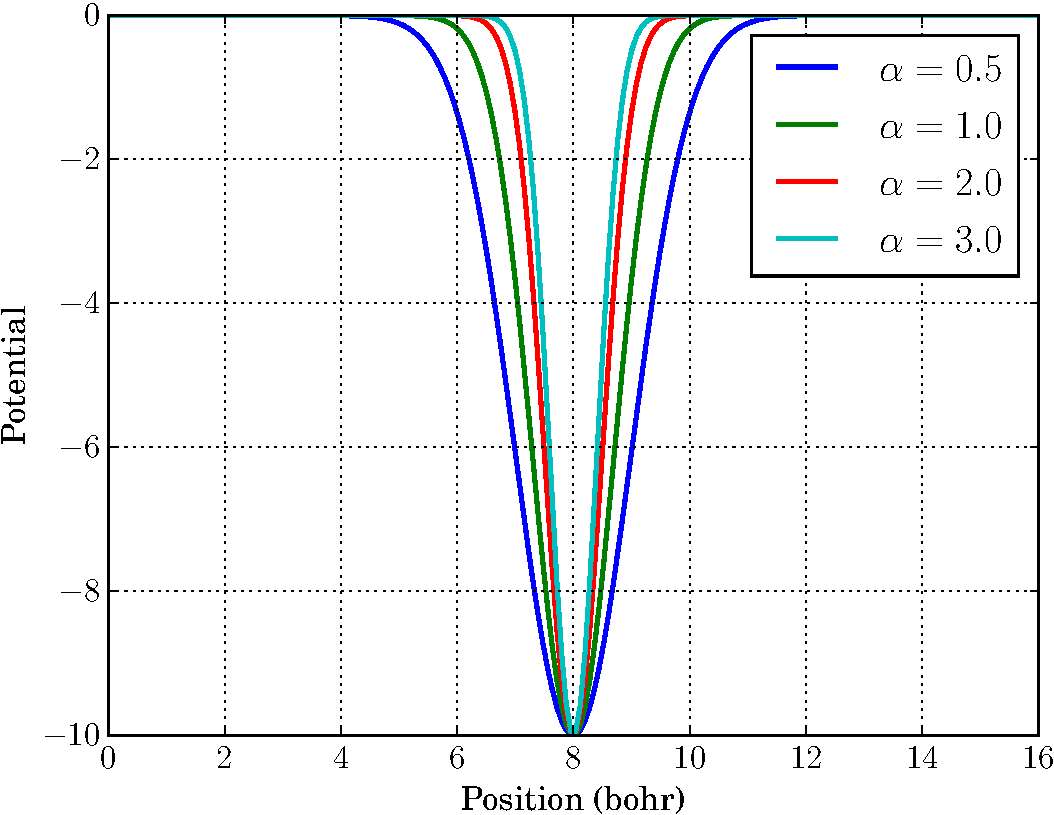
\includegraphics[width=0.5\textwidth]{images/V_gauss.pdf}
\caption{Gaussian potential}
\label{fig:gauss_pot}
\end{figure}

Result for Gaussian potential

\begin{figure*}[h]
\centering
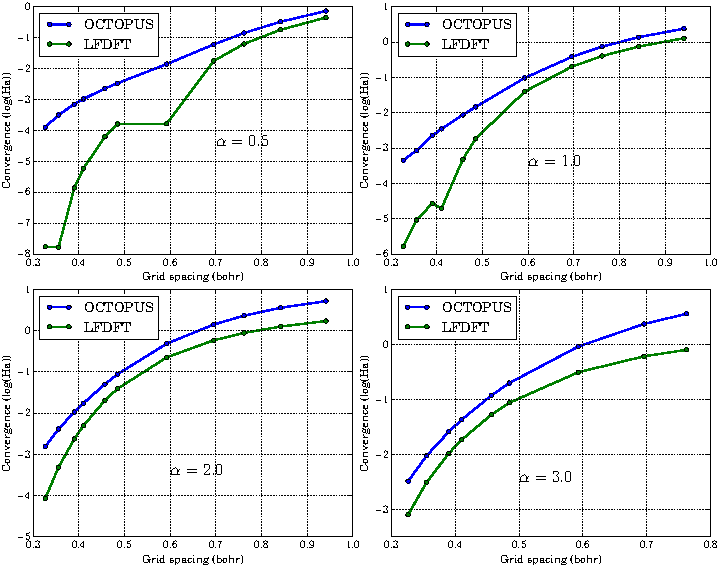
\includegraphics[scale=1.0]{images/COMBINE_v1.pdf}
\caption{Convergence}
\end{figure*}

Comparison between SCF and direct minimization:

\subsection{Hydrogen pseudopotential}

Result for atomic system

\begin{figure}
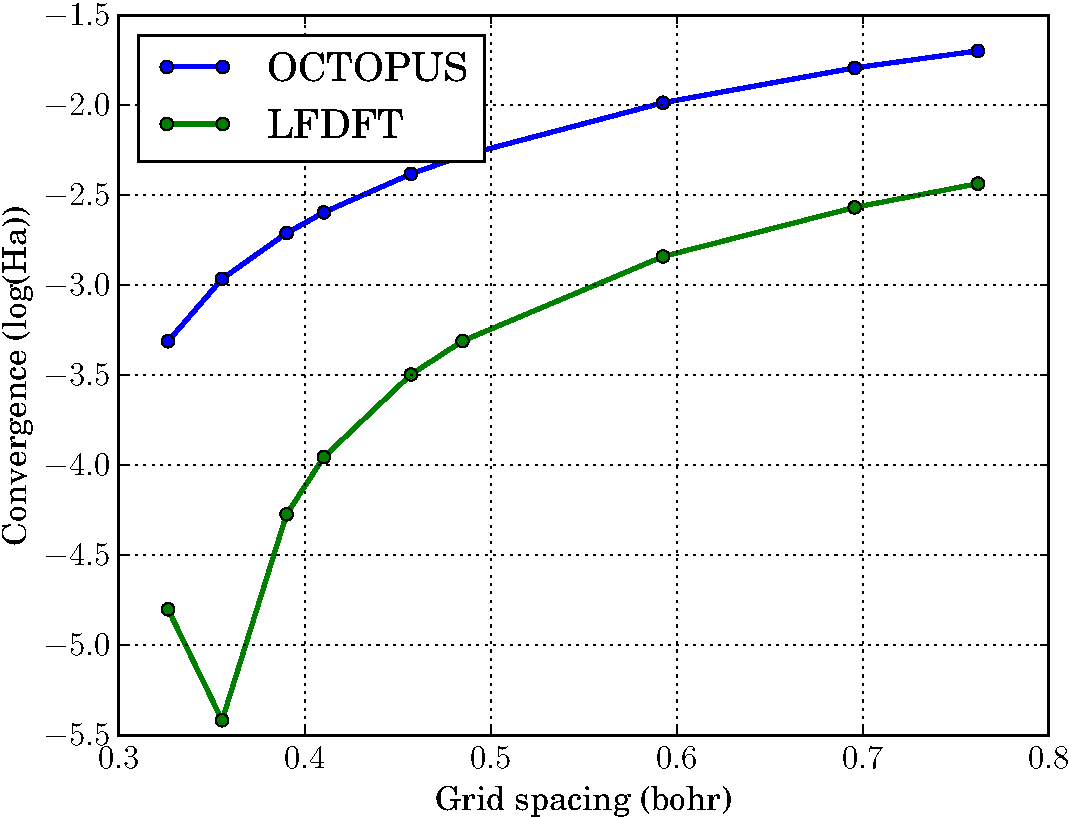
\includegraphics[width=0.5\textwidth]{images/CONV_atom_H.pdf}
\end{figure}

\subsection{Lithium pseudopotential}
Blah

